\documentclass[a4paper,11pt]{jsarticle}
\usepackage{graphicx}
\usepackage{wrapfig}
\usepackage{amsmath,amssymb,amsthm}
\usepackage{amssymb}
\usepackage{ascmac}
\usepackage{subfigure}
\usepackage{bm}
\usepackage{setspace}
\usepackage{cases}%左かっこつけるときに必要だった
\usepackage{leftidx}%行列表示用?
\usepackage{fancyhdr}
\usepackage{graphicx}
\usepackage{float}
\usepackage{booktabs}
\usepackage{url}
\usepackage{bm}
\usepackage{verbatim}
\usepackage{calc} 

\setlength{\headsep}{5mm}
\setlength{\oddsidemargin}{-0.5zw} %→にズラす
\setlength{\textheight}{37\baselineskip}
\addtolength{\textheight}{\topskip}
\setlength{\topmargin}{-10mm}
\setlength{\textwidth}{45zw} %文章の幅
\setlength{\textheight}{215mm}
\setlength{\parindent}{1zw}%箇条書きの一文字下げ
\pagestyle{fancy}

\newtheorem{theorem}{定理}
\newtheorem{prop}[theorem]{命題}
\newtheorem{lemma}[theorem]{補題}
\newtheorem{cor}[theorem]{系}
\newtheorem{example}[theorem]{例}
\newtheorem{definition}[theorem]{定義}
\newtheorem{rem}[theorem]{注意}
\newtheorem{guide}[theorem]{参考}
\renewcommand{\proofname}{証明}

\numberwithin{theorem}{section}  % 定理番号を「定理2.3」のように印刷
\numberwithin{equation}{section} % 式番号を「(3.5)」のように印刷
\newcommand{\argmax}{\mathop{\rm arg~max\,}\limits}
\newcommand{\argmin}{\mathop{\rm arg~min\,}\limits}
\newcommand{\st}{\mathop{\rm subject~to\,}\limits}
\newcommand{\sign}{\mathop{\rm sign\,}\limits}

\newcommand{\dom}{\mathop{\mathrm{\bf dom}}\nolimits}
\newcommand{\minimize}{\mathop{\mathrm{\rm minimize}}\limits}
\newcommand{\maximize}{\mathop{\mathrm{\rm maximize}}\limits}

\lhead{2012年度・CG最終レポート}
\chead{}
\rhead{12M42340}
\lfoot{チョウ シホウ}
\cfoot{\thepage}
\rfoot{6月11日}
\renewcommand{\footrulewidth}{0.4pt}
\title{2012年度・CG最終レポート}
\author{12M42340 チョウ シホウ}


\begin{document}
\pagenumbering{roman}
%\tableofcontents
%\cleardoublepage
\pagenumbering{arabic}
\renewcommand{\thepart}{\arabic{part}}

%\thispagestyle{empty}

\begin{itembox}[l]{問題1:Texturing}
\begin{enumerate}
\item
Explain {\bf aliasing} artifact of texturing from the point of view of the sampling theorem. This explanation must
have two parts. The first one is a description of the theoretical reason behind of the aliasing with equations and
illustrations. The second one is an experimental description base on the actual artifacts occurring while the animation
by the program, using snapshots of the animation.
\item Explain one texturing algorithm to avoid the artifact.
\end{enumerate}
\end{itembox}
Sourcecode:{\bf CG\_Final\_Code/MipMapping}
\begin{figure}[H]
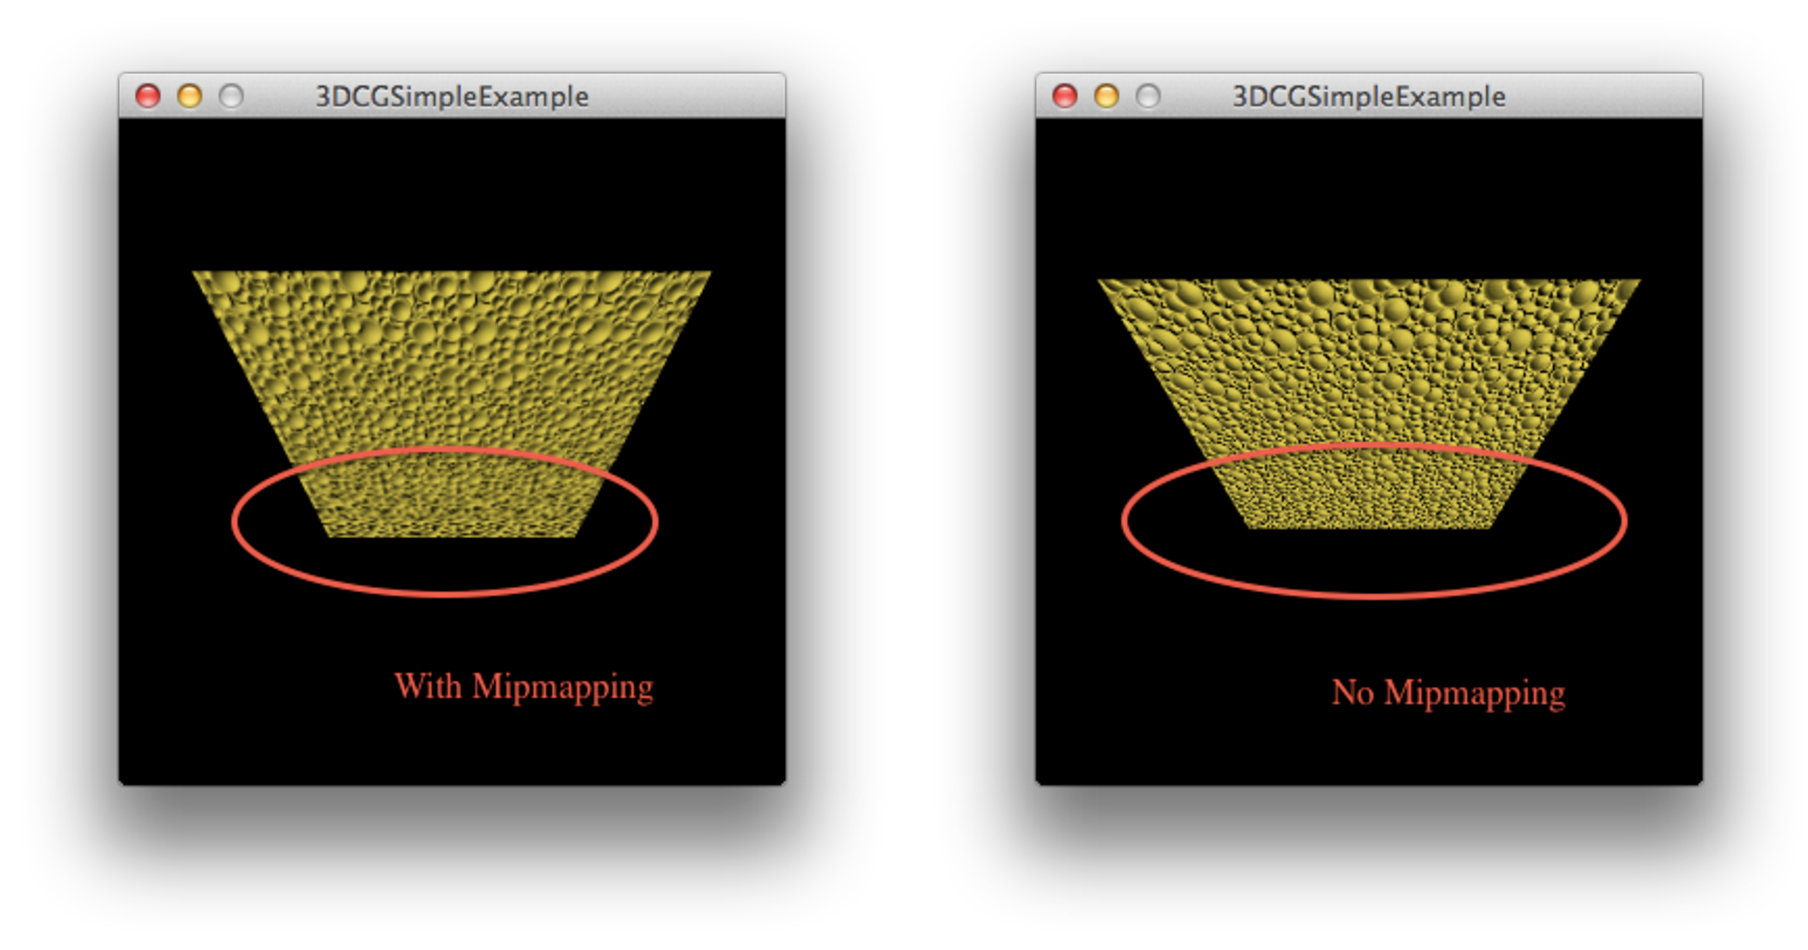
\includegraphics[bb=0 0 444 451,width=7.5cm]{mip_mapping.pdf}
\end{figure}
\newpage

\begin{itembox}[l]{問題2:Geometry Data Definition and Transform}

Define a regular icosahedron whose center is the origin and whose one edge length is $0.8$, translate the center to
$(0,0,-2)$, and make an animation that it rotates around the vertical axis which passes through the center.

Use the same framework of the program and replace the plane to the icosahedron.

Put one snapshot on your report and describe how to compile and execute your program.
\end{itembox}

Sourcecode:{\bf CG\_Final\_Code/IcosahedronNormal}

Screenshot:
\begin{figure}[H]
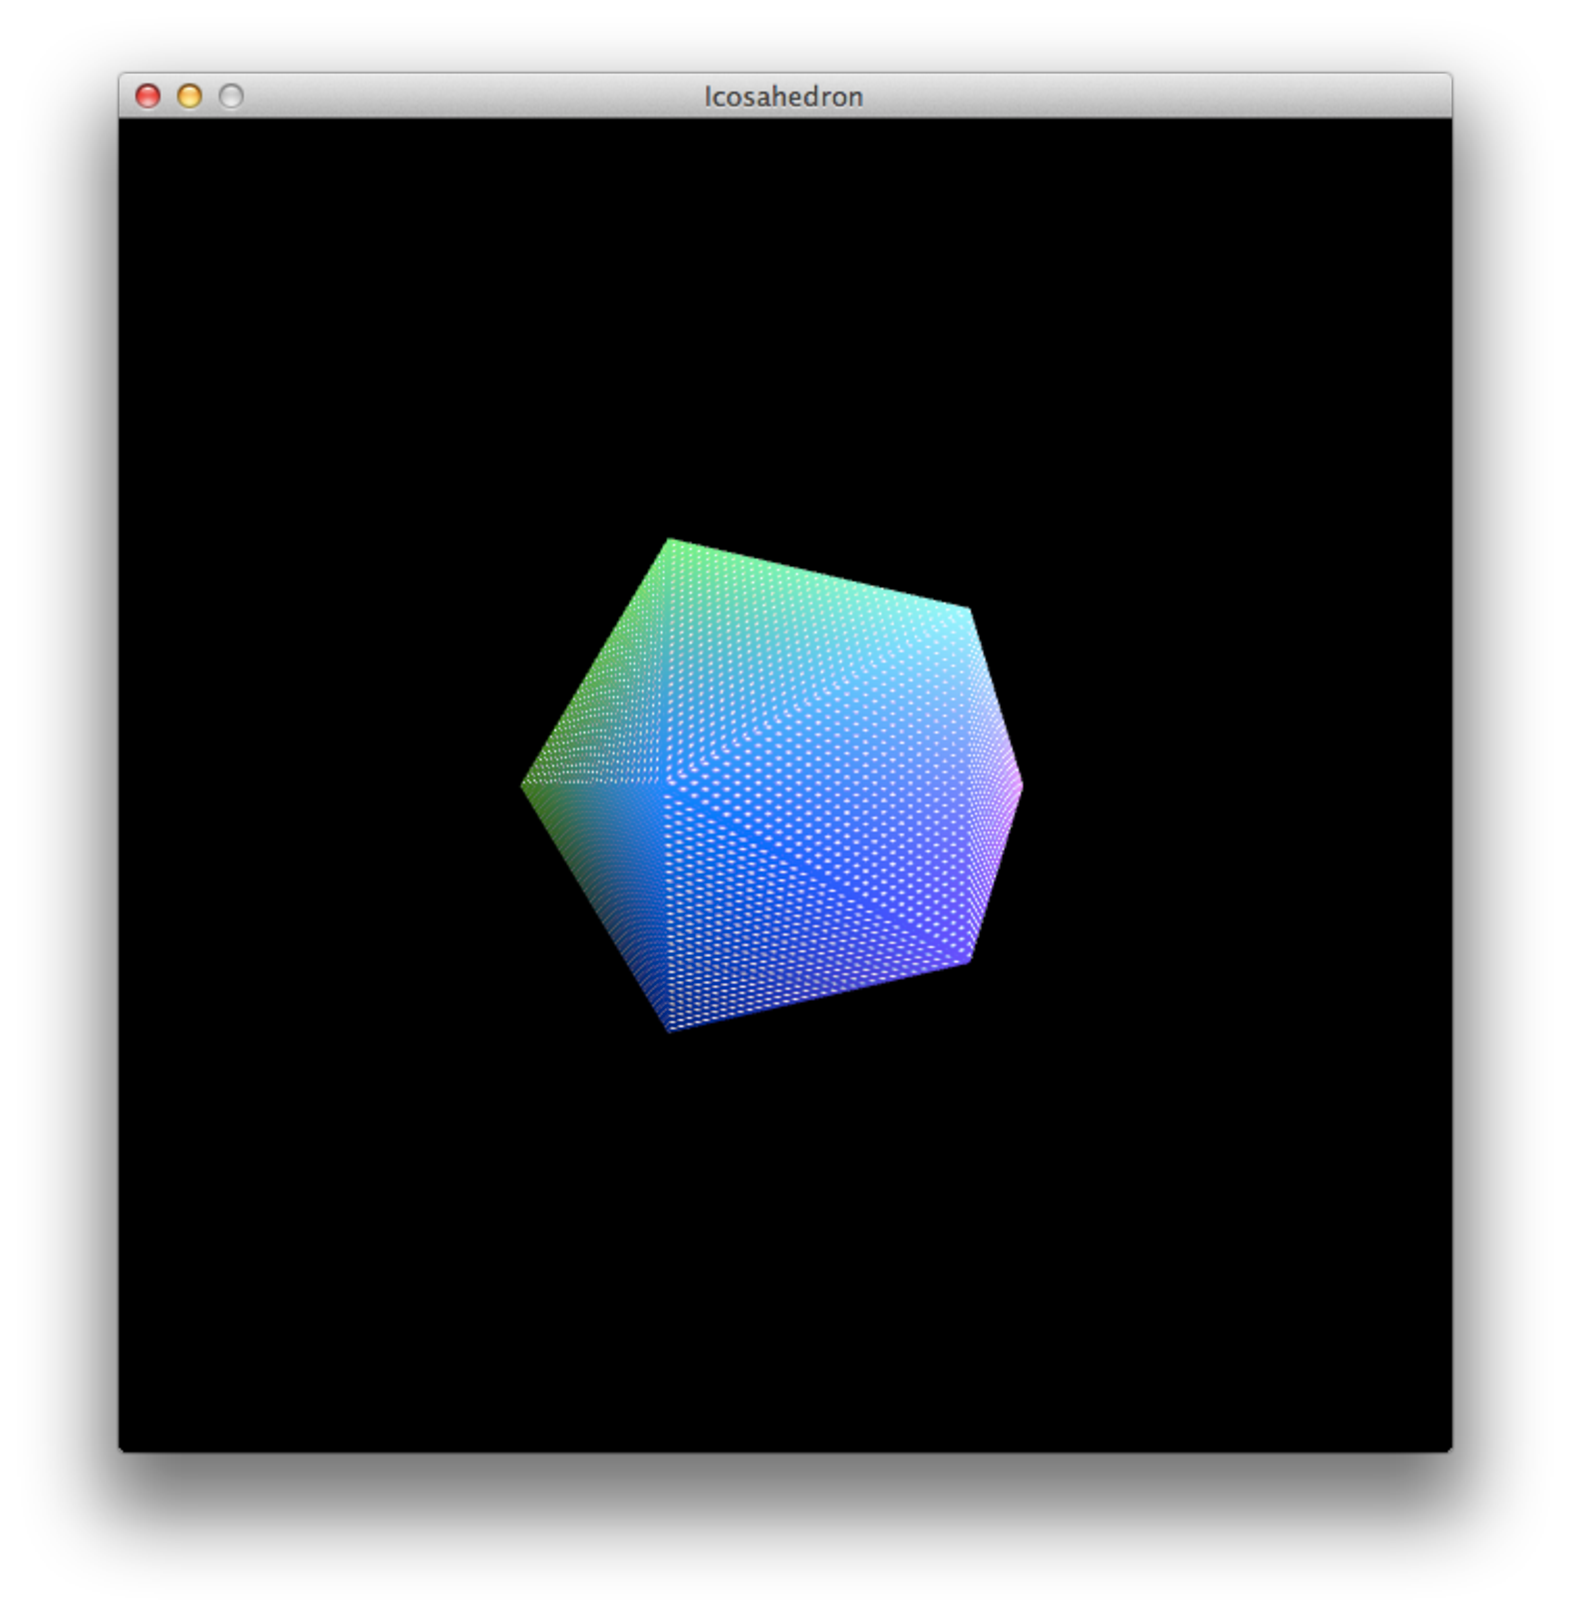
\includegraphics[bb=0 0 444 751,width=6cm]{Icosahedron.pdf}\\
\end{figure}

\newpage

\begin{itembox}[l]{問題3:Reflection}
Calculate diffuse and ambient intensities on the surface of the regular icosahedron,as if it was a sphere,in the fragment shader stage.The equation to calculate the intensities $R_{\text{rgb}}$ is defined as
\[
R_{\text{rgb}} = C_{\text{rgb}}\Bigr( \max ( - \frac{LN}{|L||N|} ) + a \Bigr)
\]
where $C_{\text{rgb}}$ is the color of
the icosahedron, $N$ is the normal vector at a point, $L$ is the vector of an incident light direction and $a$ is a coefficient of
ambient light.

Set $L$ as an efficient direction to express shading effect on the object surface.



Put one snapshot on your report and describe how to compile and execute your program.
\end{itembox}

Sourcecode:{\bf CG\_Final\_Code/IcosahedronWithReflection}

Screenshot:
\begin{figure}[H]
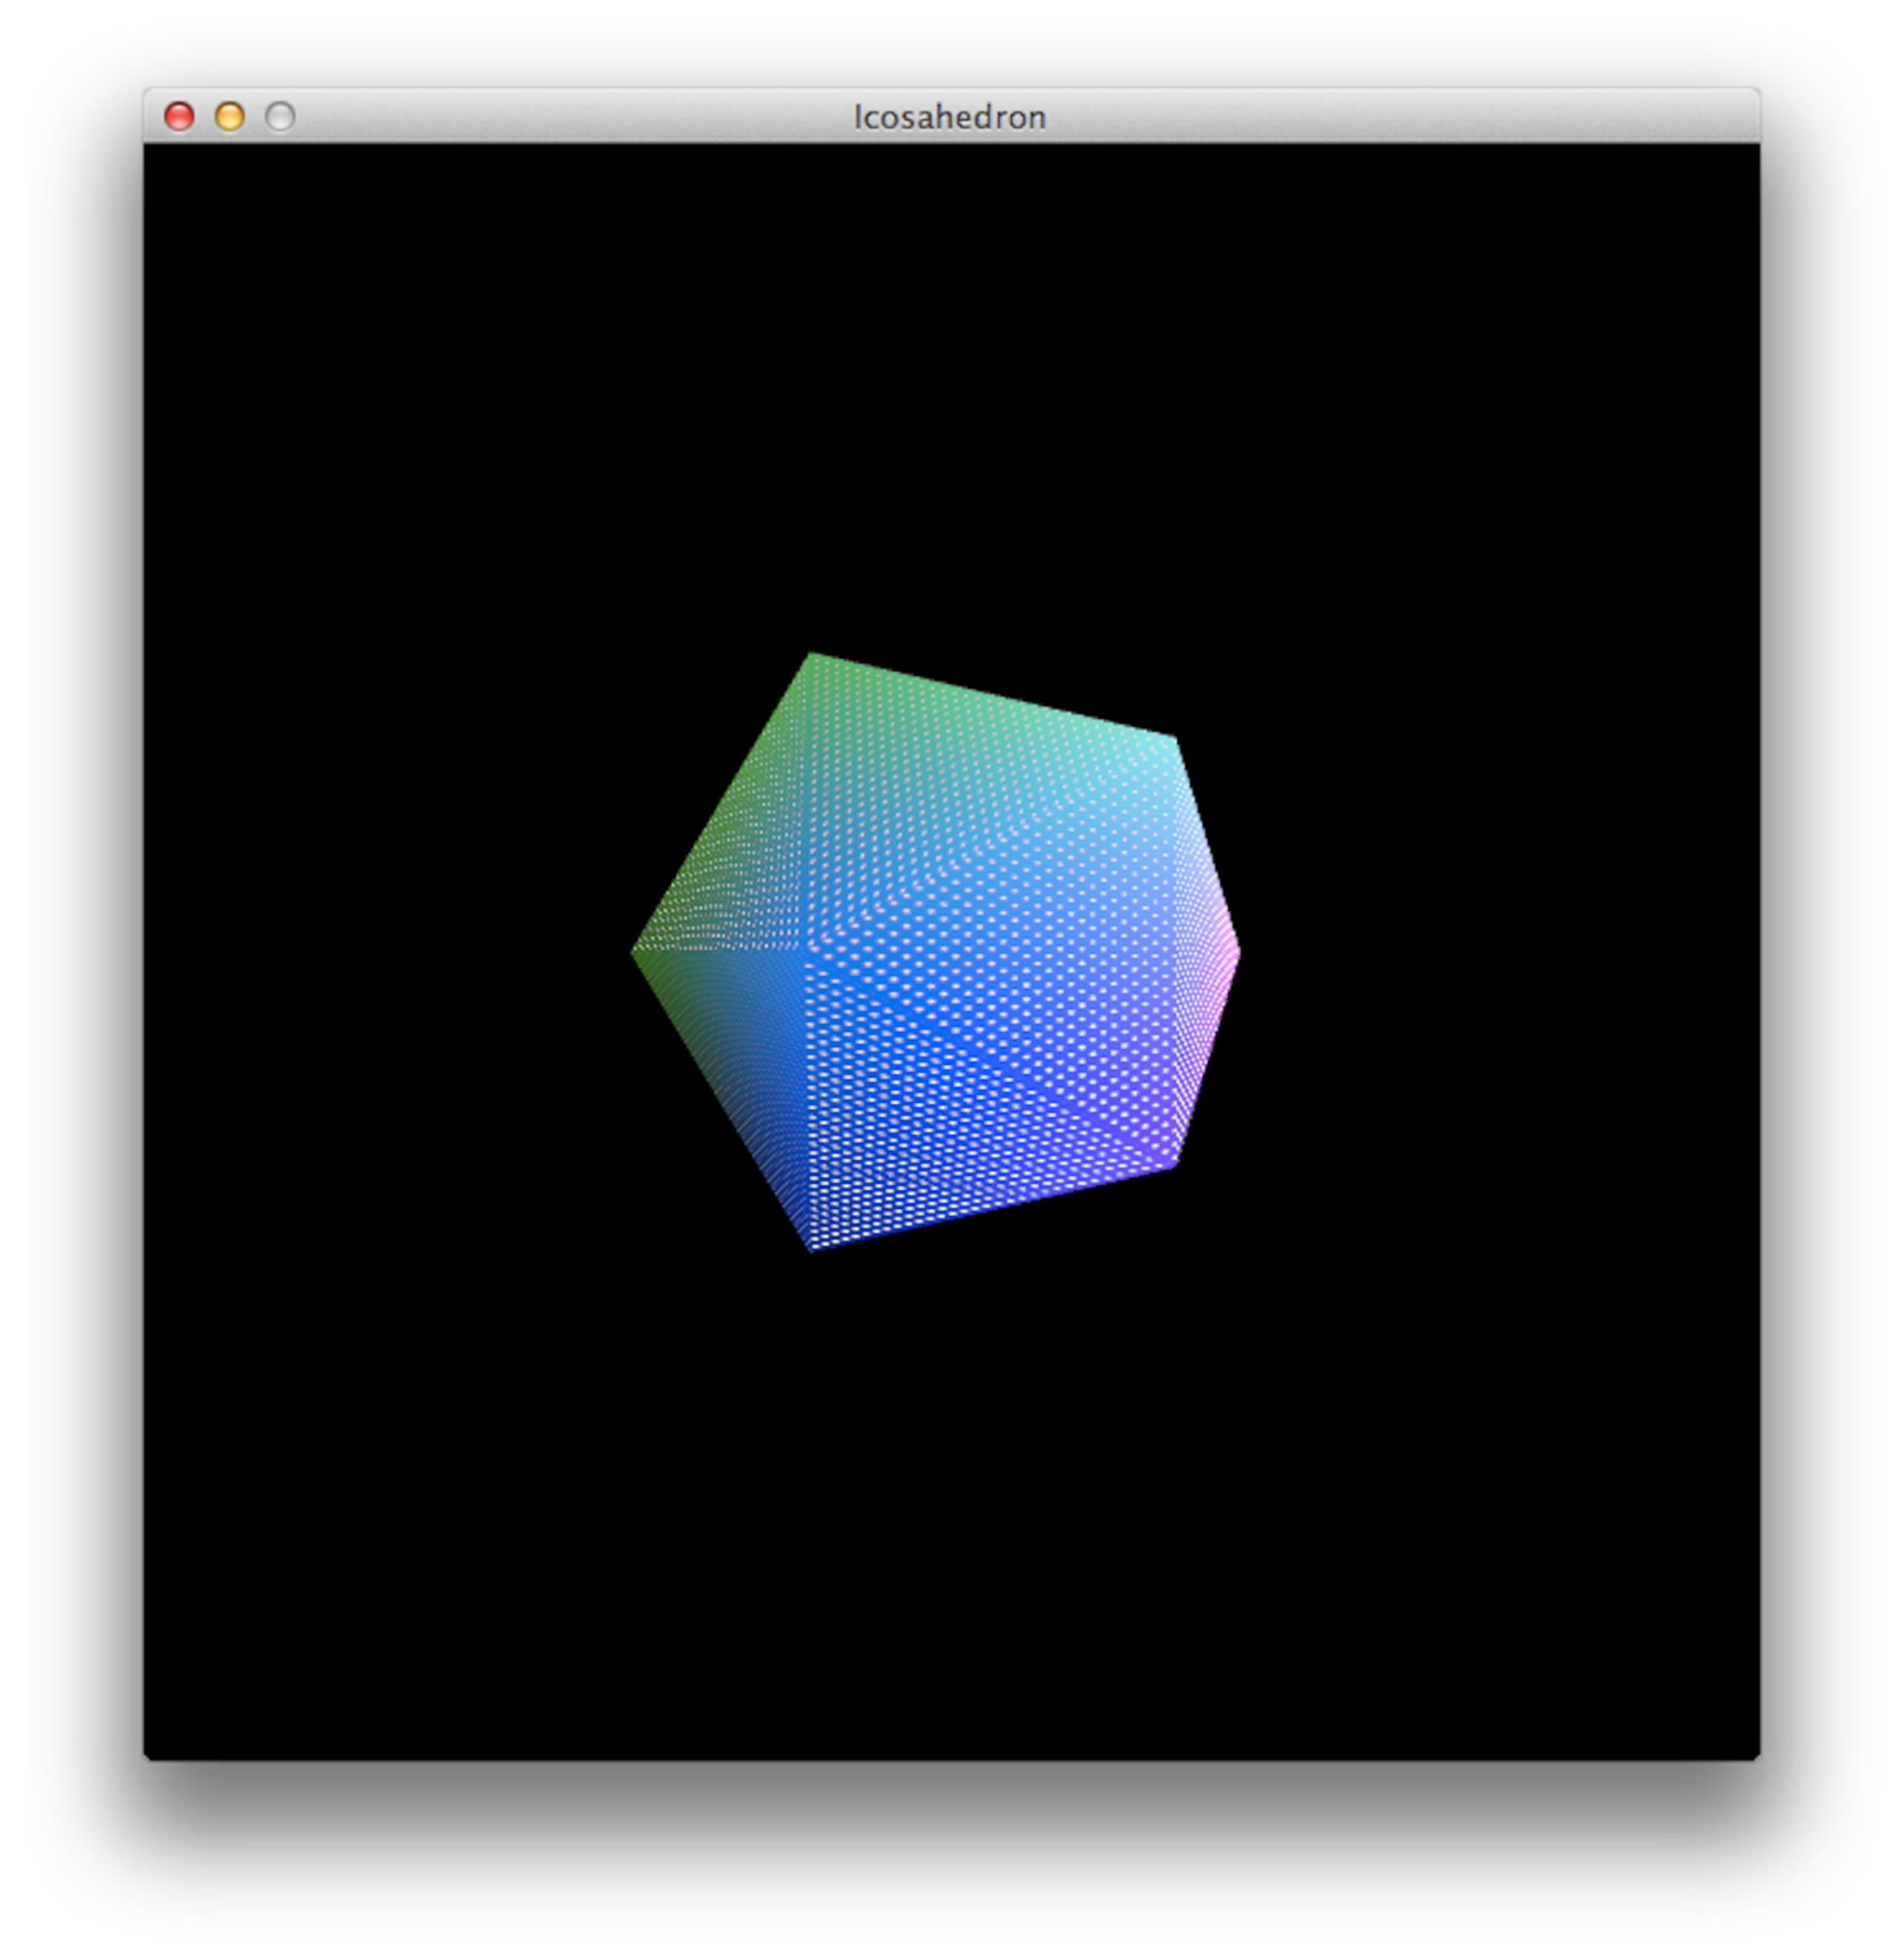
\includegraphics[bb=0 0 444 1200,width=4cm]{Icosahedron_a_and_b.pdf}
\end{figure}
スクリーンショットで示すのは,鏡面反射(光源$L=(0.0,10.0,-10.0)$)と拡散(環境光係数$a=0.5$)の組み合せです.
\begin{figure}[H]
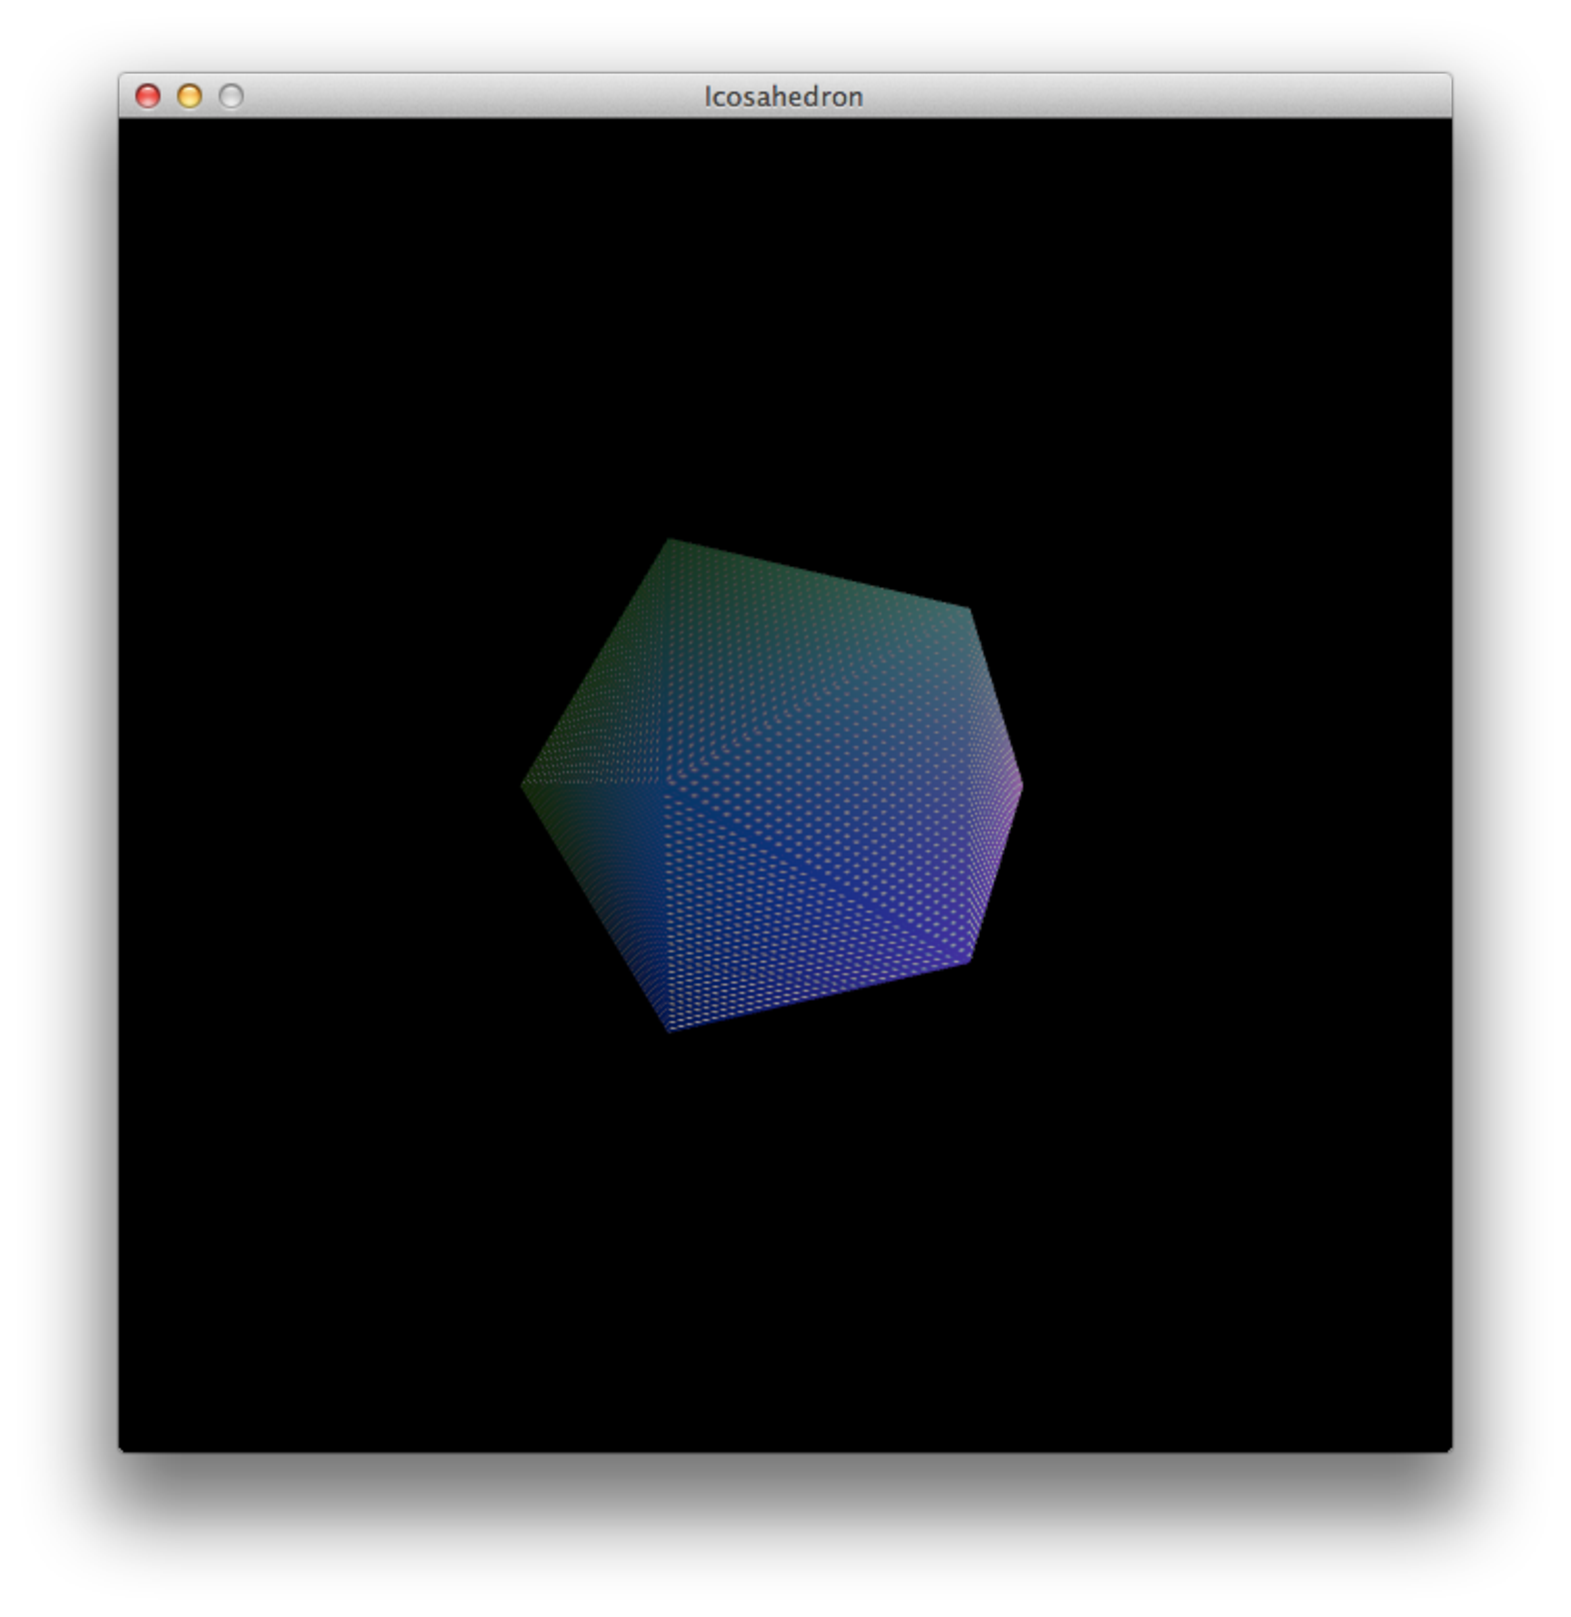
\includegraphics[bb=0 0 444 751,width=6cm]{Icosahedron_a.pdf}鏡面反射
\end{figure}
\begin{figure}[H]
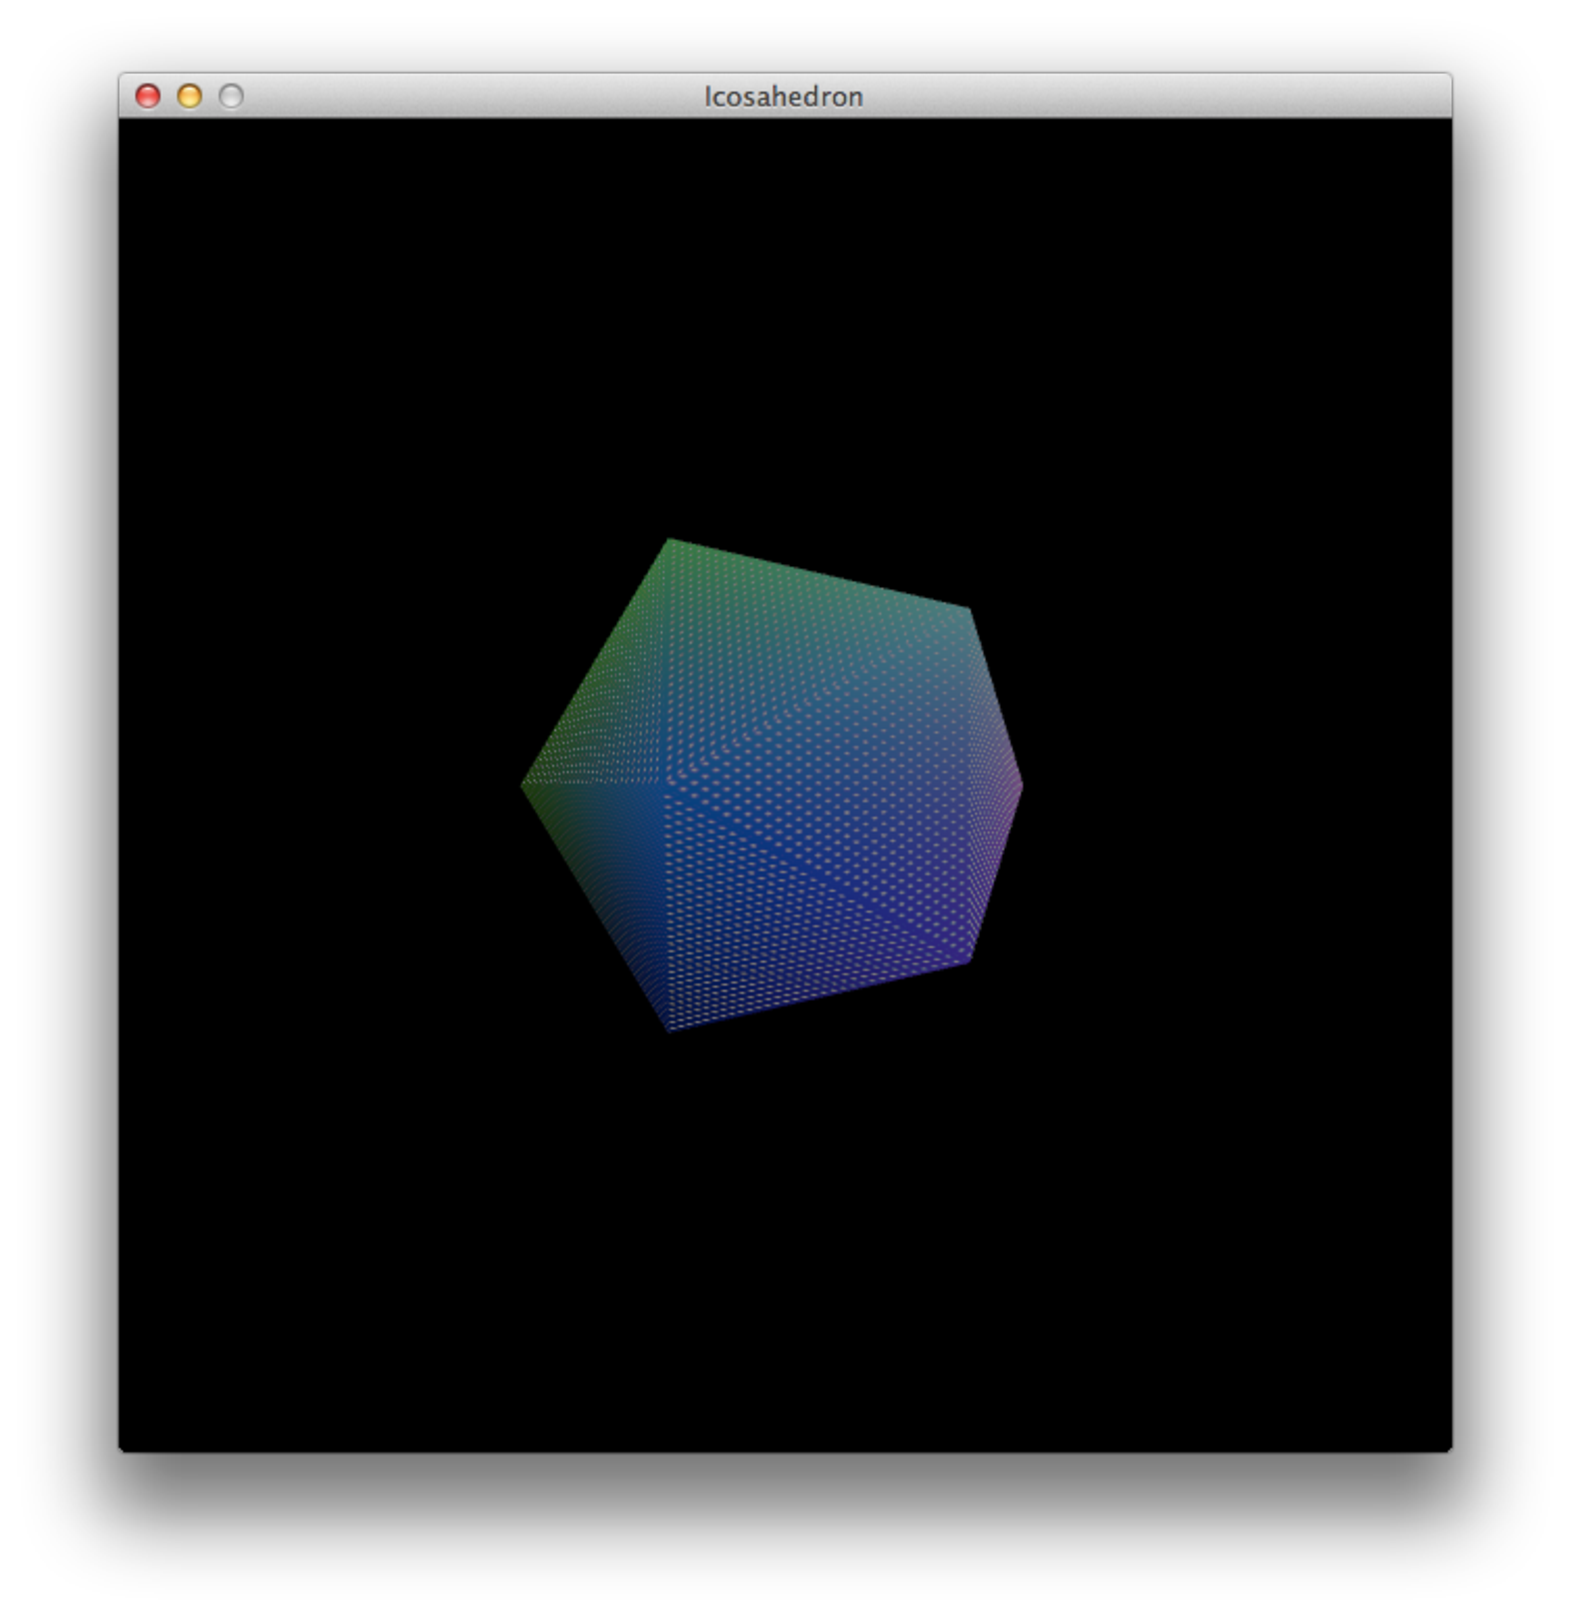
\includegraphics[bb=0 0 444 751,width=6cm]{Icosahedron_b.pdf}拡散
\end{figure}

\end{document}